\chapter{Propellant selection}
\qquad \underline{By} : Alina\\

For the propellant selection for our vehicle, several important aspects have to be taken into account including:
\begin{itemize}
	\item 	Specific impulse in vacuum (Isp) of the propellant
	\item	Storability
	\item	Toxicity including ground handling
	\item	Costs (while the main cost driver is not the propellant itself more its toxicity)
	\item	Reasonable refueling options due to the desired mission profile of the vehicle
	\item	Space flight heritage of the propellant (e.g. flight proven, ground proven or in development)
	\item	Density specific impulse
	\item	Corrosive behavior and compatibility with typical light weight tank materials as titanium or aluminum
	\item	and many more
\end{itemize}

At first several possible and typical flight proven propellant combinations were analyzed and the most promising combinations were selected and then compared in detail. Afterwards a feasibility study for the chosen propellant combination was deemed necessary in order to check whether the desired propellant combination is able to perform the required mission and de-risk the next development steps.

\section{Options overview}
\qquad In literature and historical research several reasonable and flight proven propellant combinations have been found. The propellant combinations are divided in three sub-categories: petroleum, cryogenics and hypergolic. These combinations are all bipropellant combinations, the monopropellants have already been excluded at the beginning due considerably low specific impulse in comparison to bipropellants and therefore not suitable for the intended mission profile.\\

Petroleum fuels are containing a combination of complex hydrocarbons and have been refined from mineral oil. The typical petroleum used as rocket fuel is a highly refined kerosene, called RP-1 (rocket propellant 1). In bipropellant use an oxidizer is necessary and therefore petroleum is often mixed with LOX (liquid oxygen). The specific impulse of a petroleum fuel and cryogenic oxidizer combination is higher than for hypergolic propellant combinations but lower than for fully cryogenic options. \\

The cryogenics are gaseous bipropellants stored at very low temperatures and usually stand out due to their high specific impulse. The most common cryogenics are liquid hydrogen and liquid oxygen which have to be stored at $-253^\circ$C for LH2 and $-183^\circ$C for LOX. Recently, cryogenic combinations with liquid methane (LCH4) as fuel are receiving more attention due to availability methane on mars and therefore it might become attractive for future mars missions.\\

The last group in this option overview are the hypergolics. The hypergolics are bipropellants that ignite spontaneously when in contact. The main advantage of hypergolics is the storability. Hypergolics are liquid at room temperature and therefore no additional heating or cooling is necessary during the mission. Nevertheless the hypergolics provide less specific impulses than cryogenics and they are mostly highly toxic.\\

\autoref{tab1} shows a comparison of different bipropellants divided in the three above mentioned categories. In the initial comparison of this chapters the propellant combinations are compared with regards to their major characteristics: specific impulse, flight evidence and therefore technical risk, storability and their reasonability for our application. \\

It is clearly visible that most propellant combinations have not been found reasonable for our application due to low temperature storage. Our vehicle is designed to perform several missions with several ignitions permission and refueling at an in orbit refueling station – this mission profile is not conformable with constant low temperature storage. \\

In contrast to that the group of hypergolics offers great storability and good specific impulse for the mission profile and a storage of these propellants at an in orbit refueling station is feasible. Since the two options MON/MMH and H2O2/RP-1 are promising, further in depth analysis was deemed necessary. 
\begin{table}[H]

	\centering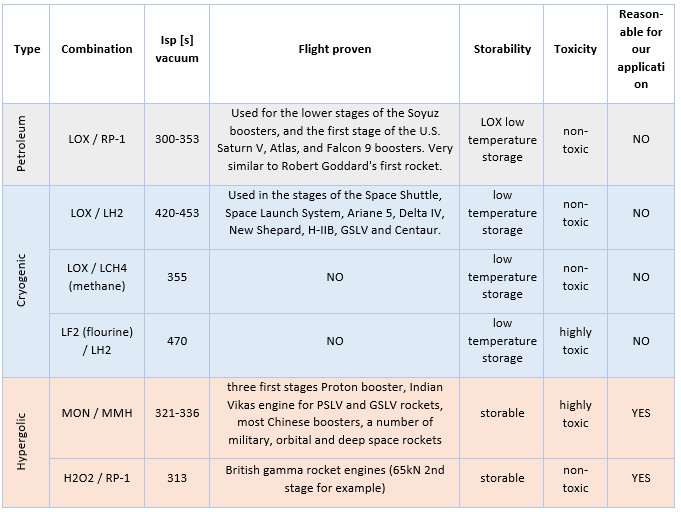
\includegraphics[width=\linewidth]{propcombination}
	
	\caption{Propellant combinations overview}\label{tab1}
\end{table}

\section{Detailed comparison between MON/MMH and H2O2/RP-1}
\qquad The hypergolic propellant combination MON/MMH and H2O2/RP-1 have been found reasonable for our mission and application. \autoref{tab2} shows a detailed comparison of the propellant combinations. Several characteristics were found to be minor and others were found to be major for our application. The major characteristics are the vacuum specific impulse, the tank volume ration, the combined density, the density specific impulse and the toxicity and storability (highlighted in yellow). \\

Both propellant combinations have a comparable specific impulse. Therefore no favor for either MON/MMH or H2O2/RP-1.\\

The tank volume ratio is better for MON/MMH because the ratio is nearly one to one, therefore both oxidizer and fuel tank could share the same tank design. This would significantly decrease the development costs since no second tank design and second qualification tank is necessary. Also the manufacturing costs would decreased due to more possibilities of batch production. Especially production costs of forged tank hemispheres are a huge cost driver and these would decrease due to non-recurring costs being distributed on a larger number of hemispheres.  Also the costs for jigs and tools would decrease. This favors MON/MMH.\\

The combined density for H2O2/RP-1 is slightly better than for MON/MMH. Nevertheless the combined density is not a significant value without taking the specific impulse into account. Calculating the density specific impulse, which is basically the specific impulse per mass, H2O2/RP-1 exceeds MON/MMH by 12\%. In this category H2O2/RP-1 is the winner because it can provide more specific impulse per mass.\\

Comparing toxicity of MON/MMH to H2O2/RP-1 it can be stated that MON/MMH is highly toxic and has to be handled with extreme care which increases the ground handling costs of this propellant combination. In contrast to that is the toxicity of H2O2/RP-1. This propellant combination is non-toxic and can be considered as “green” propellant. Nevertheless careful ground-handling is also necessary for this combination because it is prone to reaction with trace elements. H2O2/RP-1 succeeds in this category.\\

The last category is the storability. Since both propellant combinations are storable in liquid/liquid condition both propellants are suitable for the application.\\

Taking all criteria and results into account H2O2/RP-1 is the preferred propellant combination for our application. The main reasons are:
\begin{itemize}
	\item	comparable specific impulse to MON/MMH
	\item	better density specific impulse
	\item	non-toxic advantage for maintenance at refuel station
	\item	good on-ground handling
	\item	possibility of R\&D funds by ESA for green debris remover	
\end{itemize}

The main reason against MON/MMH is the toxicity.

\begin{table}
	\centering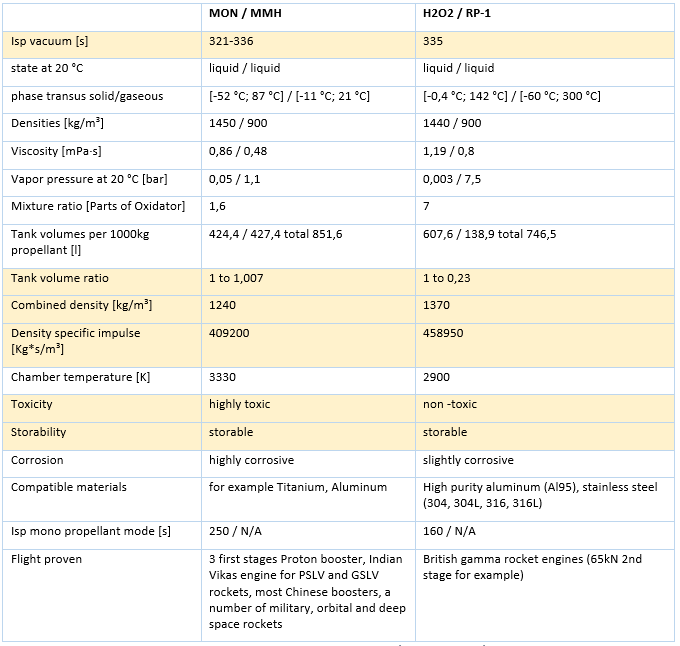
\includegraphics[width=\linewidth]{detailedcompprop}
	\caption{Detailed propellant comparison MON/MMH and H2O2/RP-1}\label{tab2}
\end{table}
\section{H2O2/RP-1 feasibility check}
\qquad Since H2O2/RP-1 is not a common propellant combination and not as frequently used space industry as MON/MHH a further feasibility study has to be performed:

\begin{itemize}
	\item	to de-risk the next development steps
	\item	to check whether the desired propellant combination is able to perform the required mission
\end{itemize}

In \ref{tab3} historical data of flight H2O2/RP-1 engines is analyzed. One of the engines “Gamma-2” was flown, the others were in development. The thrusts of all engines are comparable or higher than foreseen for our application and two engines also operate in comparable delta-v ranges. This leads to the conclusion that a H2O2/RP-1 engine is generally speaking feasible.

\begin{table}
	\centering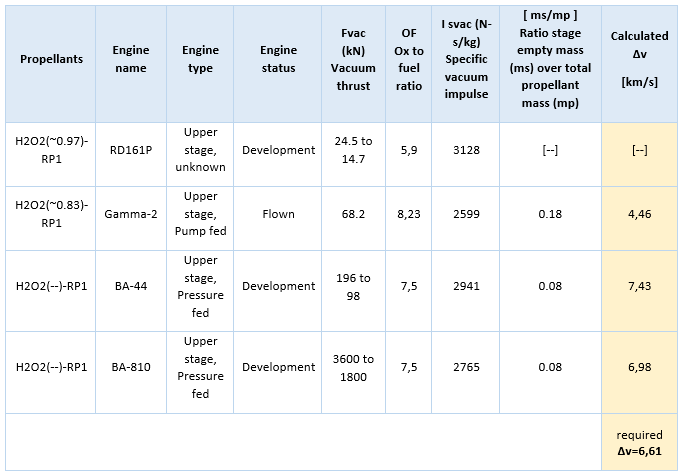
\includegraphics[width=\linewidth]{histflightprop}
	\caption{Historical data of flight H2O2/RP-1 engines}\label{tab3}
\end{table}
\section{Summary}

\qquad In summary H2O2/RP-1 is a viable non-toxic hypergolic propellant combination with a good density specific impulse. Additionally the propellant combination is supported by historical flight data. Therefore all further steps will be based on this combination.